\section{Overview}

    \begin{comment}
    
    In this problem, a sequence of contiguous real values between 0.0 and 1.0 are generated. Given one or more time steps of past values, the model must predict the next item in the sequence.
    
    Sequence prediction problems have been around for a long time. They are considered as one of the hardest problems to solve in the data science industry. These include a wide range of problems; from predicting sales to finding patterns in stock markets’ data, from understanding movie plots to recognizing your way of speech, from language translations to predicting your next word on your iPhone’s keyboard.
    
    With the recent breakthroughs that have been happening in data science, it is found that for almost all of these sequence prediction problems, Long short Term Memory networks, a.k.a LSTMs have been observed as the most effective solution.
    
    LSTMs are a very promising solution to sequence and time series related problems. 
    
    Data is prepared in a format such that if we want the LSTM to predict the ‘O’ in ‘HELLO’  we would feed in [‘H’, ‘E‘ , ‘L ‘ , ‘L‘ ] as the input and [‘O’] as the expected output. Similarly, here we fix the length of the sequence that we want (set to 50 in the example) and then save the encodings of the first 49 characters in X and the expected output i.e. the 50th character in Y.
    
    A LSTM network expects the input to be in the form [samples, time steps, features] where samples is the number of data points we have, time steps is the number of time-dependent steps that are there in a single data point, features refers to the number of variables we have for the corresponding true value in Y. We then scale the values in X_modified between 0 to 1 and one hot encode our true values in Y_modified.
    
    We will use the library Keras, which is a high-level API for neural networks and works on top of TensorFlow or Theano. So make sure that before diving into this code you have Keras installed and functional.
    
    LSTMs have an edge over conventional feed-forward neural networks and RNN in many ways. This is because of their property of selectively remembering patterns for long durations of time.  The purpose of this article is to explain LSTM and enable you to use it in real life problems.  Let’s have a look!
    
    \end{comment}
    \begin{comment}
    
    - Methodology
        - Luria ->  
            -> Sequence 
            -> Pattern 
            -> Patterns have mistakes 
                (Figure ref) 
            -> Mistake 
            -> Anomaly
            
        - Predict next expected value, based on previous value
        - Train Neural Network to handle task
        - Measure difference 
        - Detect Anomaly
        - Generate features
        
    - Sequence Extraction
        - n normal drawings
    
    - LSTM neural network background
    - Input generation
        - Sliding window based sequence to n-dimensional data transformer
    
    - LSTM training
    - Anomaly detection
        - Entities used: 
            Drawing, Edge, Anomaly, LSTM container, LSTM model
    - Anomaly Features
        - Anomaly X count in Edge at d=0
        - Anomaly X count in Drawing
    
    
    % Proposed anomaly detection solution may include following important aspects. Should exist logic for sequence extraction from Drawing entity. Sequence should be represented by numeric vector and also should be meaningful in the context of our research.
    % It is also required to train neural network NN model to reproduce normal sequences without mistakes. 
    
    pted to back some of these intuitions with
    experimental results. We have also presented new insights, both
    on architecture selection and hyperparameter tuning for LSTM
    networks which have emerged as the method of choice for
    solving complex sequence learning problems. In future work,
    we plan to explore more complex modifications of the LSTM
    architecture.
    
    % After last phase of the implementation, different types of features were extracted from processed Drawing objects. 
    % Current research subject is set of drawings of Luria pattern from different groups of individuals: healthy controls and Parkinson's disease patients. Pattern itself is... 
    
    % In the natural sciences an anomaly is the deviation in a quantity from its expected value, e.g., the difference between a measurement and a mean or a model prediction. Similarly, a standardized anomaly equals an anomaly divided by a standard deviation.[1] A group of anomalies can be analyzed spatially, as a map, or temporally, as a time series. There are examples in atmospheric sciences and in geophysics.
    
    \end{comment}

Motivation behind proposed anomaly detection solution based on following assumptions. Current research subject is essentially a Luria pattern drawing. Pattern itself is sequence of repetitive groups of elements. It is expected, that tested individuals, while drawing a pattern, may produce mistakes. Healthy subjects, by intuition, should produce less mistakes, than subjects with \textit{PD}, therefore mistake detection may have potential in Parkinson's disease prediction.

Mistakes can be interpreted as anomalies. An anomaly, by definition, is an element in the sequence with significant deviation from its expected value \cite{chandola2009anomaly}. Expected value can be obtained from average value of similarly positioned elements of the sequence. Another option --- is to obtain expected value from sequential model prediction. 

Upper chart on Figure \ref{sequence-angle} illustrates \textit{normal} behaviour of the \textit{angle} sequence from the subset of \textit{normal} \textit{Drawings}. Lower chart is subset of \textit{Drawings} with \textit{anomalies}. Similarity between different sequences within  \textit{normal} subset is obvious, therefore it is possible to construct sequential neural network NN model, capable of reproducing comparable signal.

\begin{figure}[htb]
  \centering
    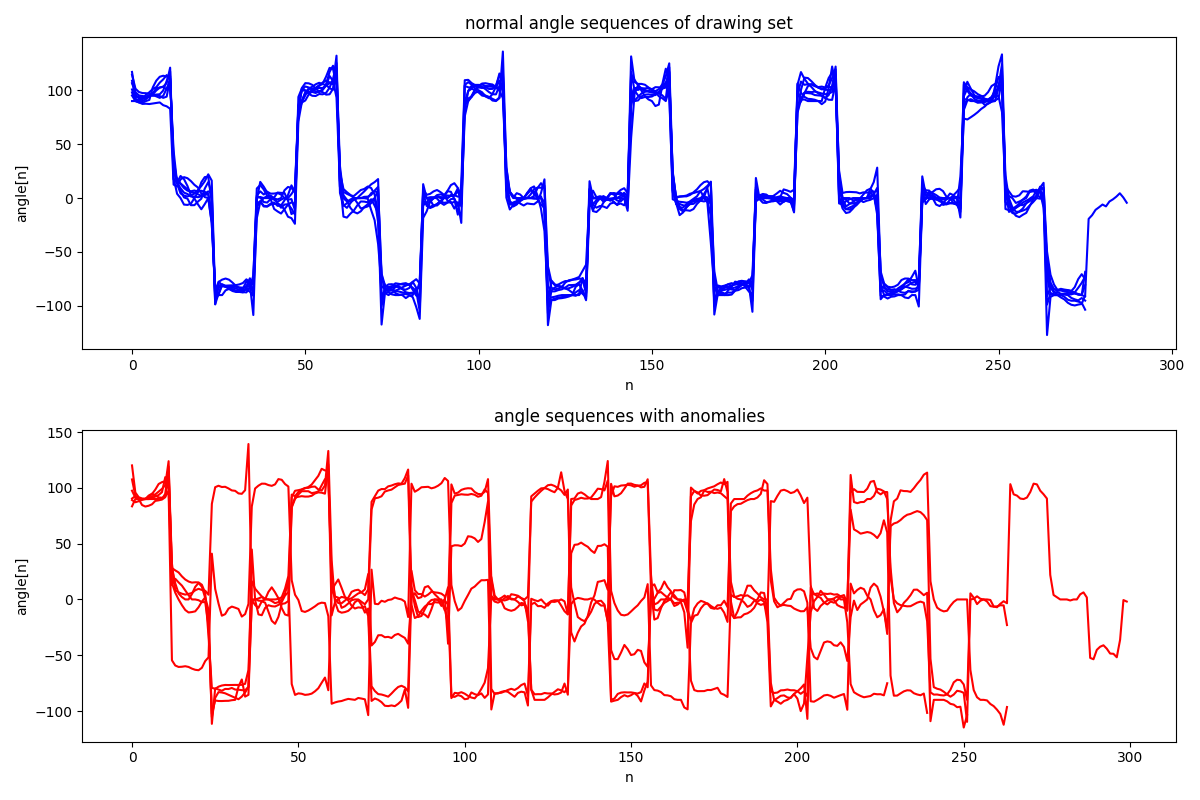
\includegraphics[width=0.99\textwidth]
        {images/anomaly/sequence-angle}
    \caption{Combined Sequences of 'Angle' Feature --- \textit{Normal} Subset (Upper Chart) and Subset with \textit{Anomalies} (Lower Chart)}
    \label{sequence-angle}
\end{figure}

Proposed \textit{anomaly detection} solution includes following important steps:

\begin{easylist}[itemize]

& \textit{Sequence Extraction} --- logic for \textit{sequence} extraction from Drawing entity. \textit{Sequence} essentially is vector of separate numeric feature $x$ of the \textit{Edge} entity of the Drawing object. Sequence is represented by vector $[x_1, x_2...x_n]$

& \textit{Neural Network Training} --- neural networks NN have proven high efficiency in sequential data processing. NN model should be able to reproduce normal sequence of feature $x$ with low error rate.

& \textit{Anomaly Detection} --- process consists from two sub-processes:
&& \textit{Sequence Prediction} --- predict sequence $[y_1, y_2...y_n]$ from existing sequence $[x_1, x_2...x_n]$ of arbitrary Drawing feature $x$.

&& \textit{Error Evaluation} --- Compare original sequence $[x_1, x_2...x_n]$ with predicted $[y_1, y_2...y_n]$, evaluate elements with significant difference, generate \textit{anomaly} objects.

& \textit{Anomaly Feature Generation} --- generate numeric features from generated \textit{anomalies} for subsequent analysis.

\end{easylist}

\section{Important Components}

\subsection{Sequence Extractor}

\begin{figure}[htb]
  \centering
    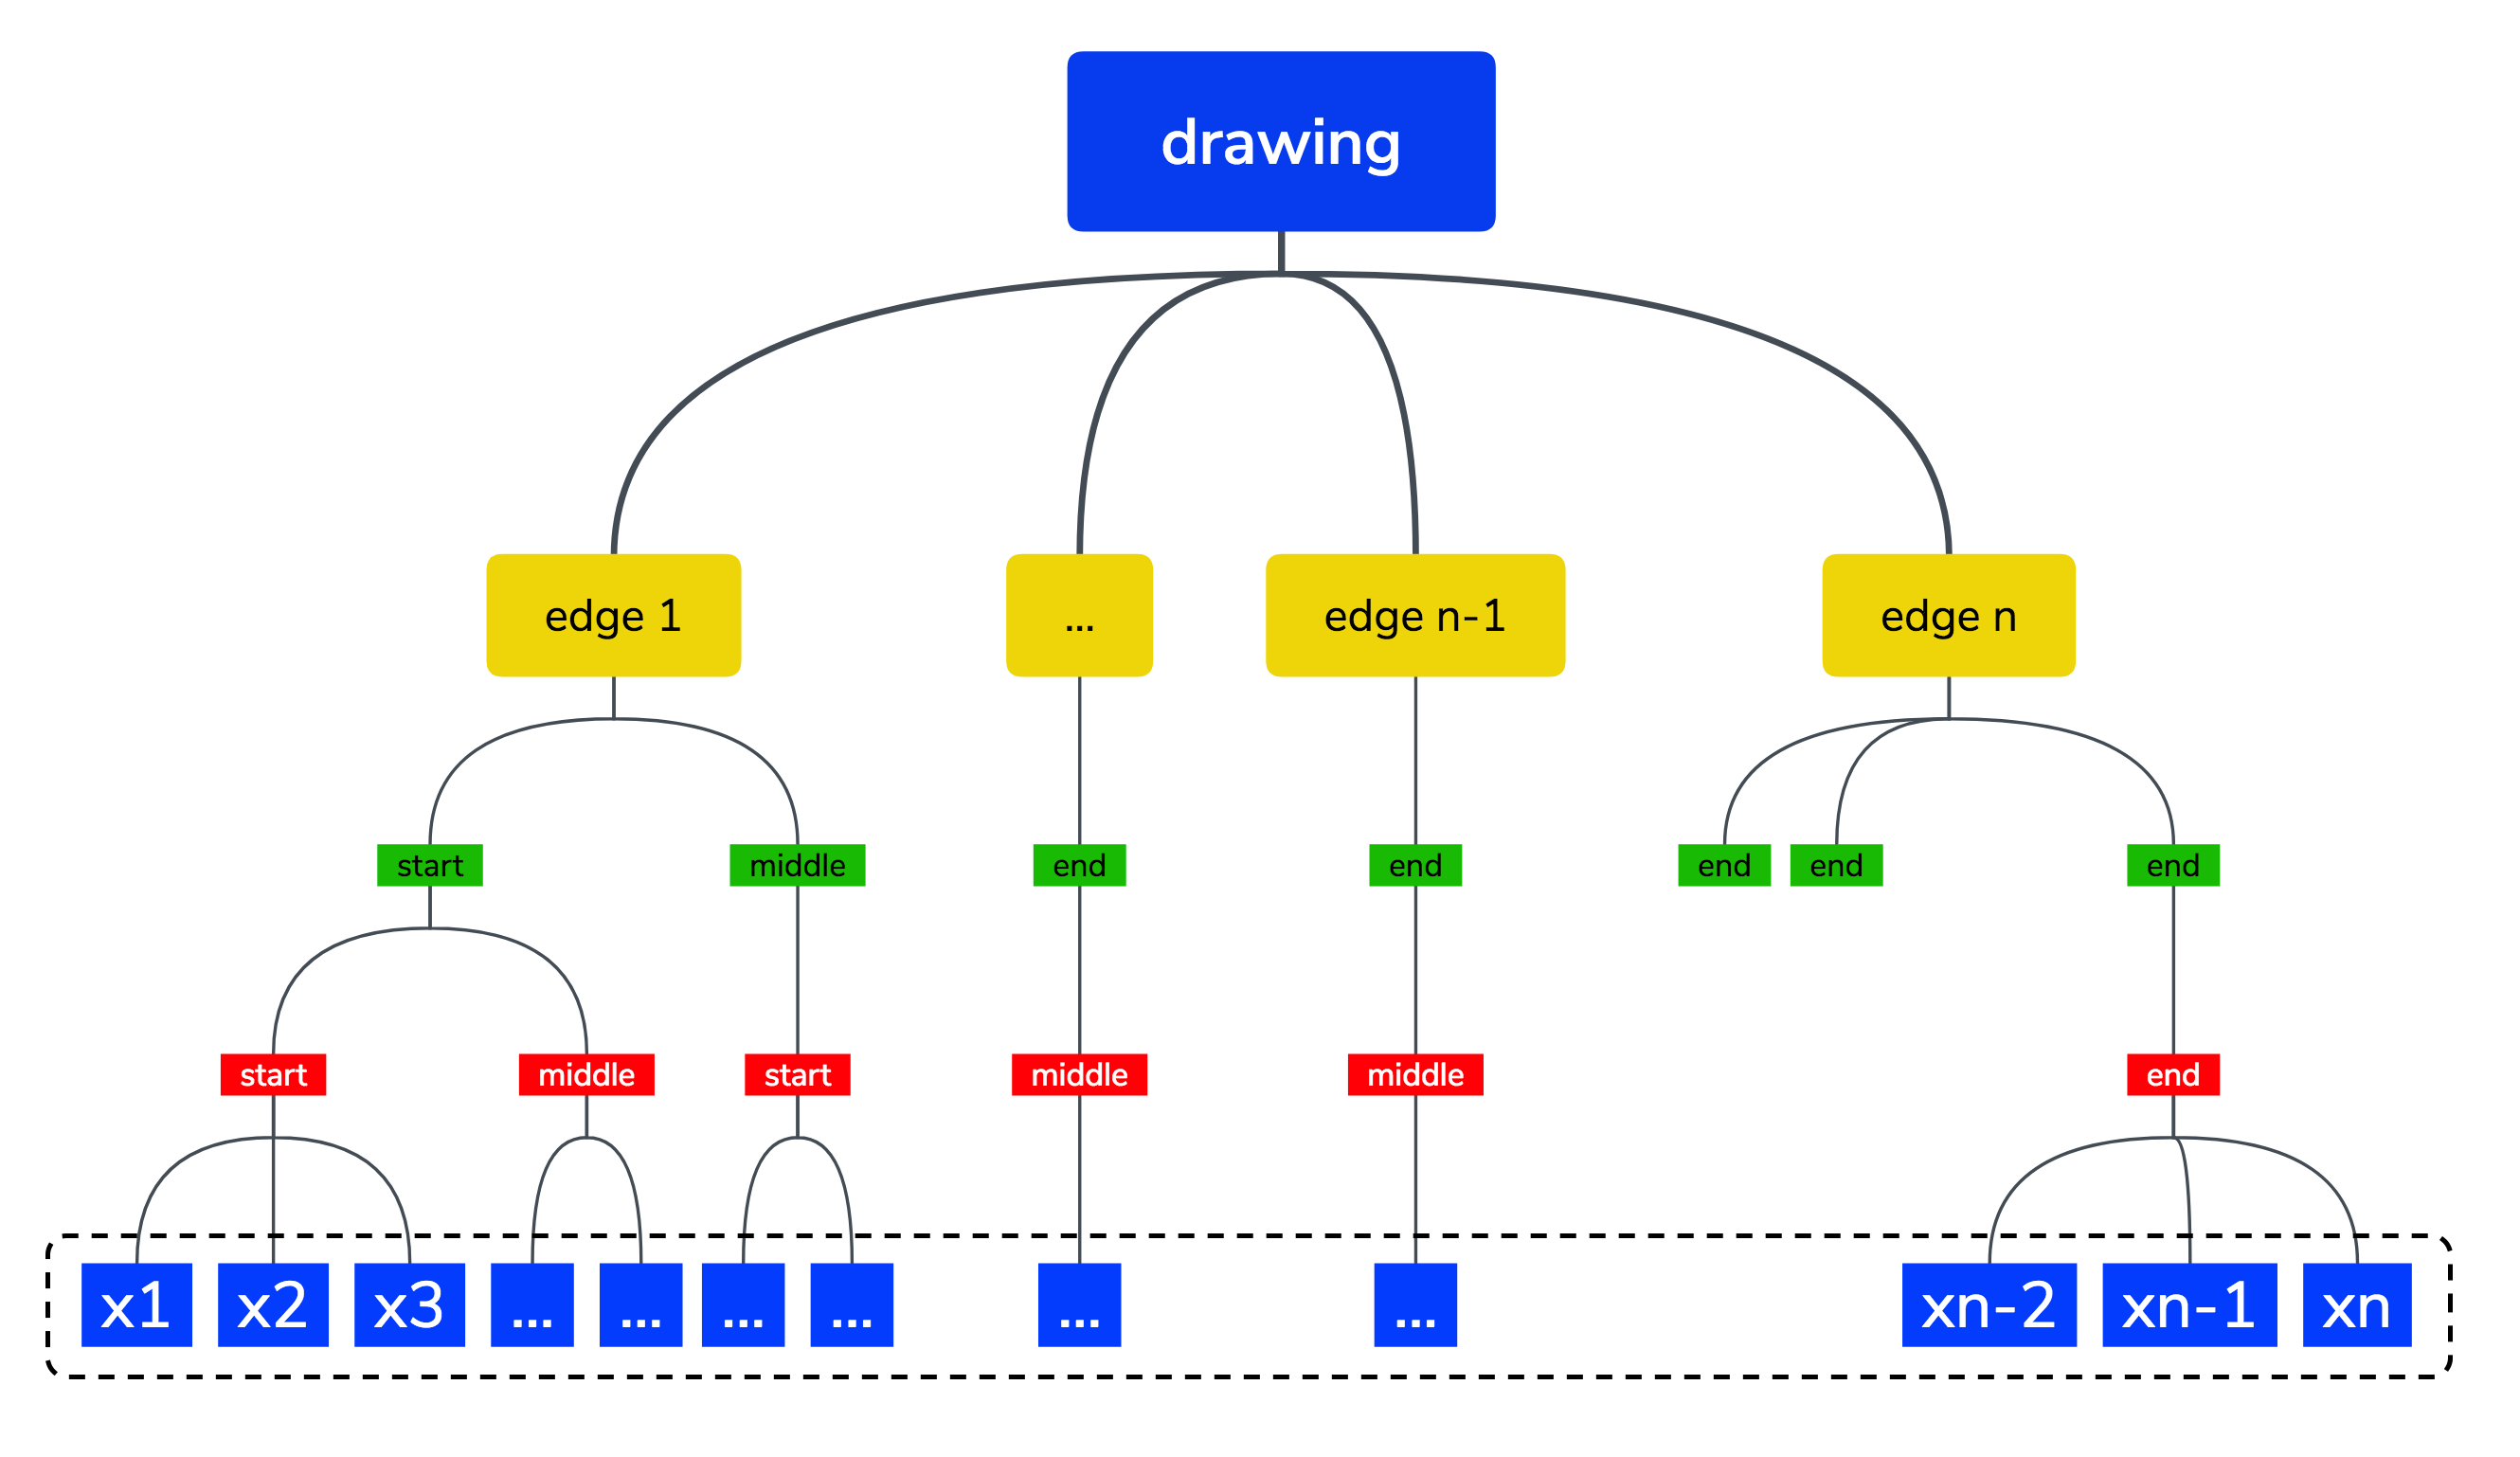
\includegraphics[width=0.75\textwidth]
        {images/anomaly/sequence-graph}
    \caption{Sequence of arbitrary feature $x$ extracted from \textit{Edge} graph at depth $d=4$ represented by vector $[x_1, x_2...x_n]$ }
    \label{sequence-graph}
\end{figure}

After previous phases of algorithm, we've already acquired set of Drawing entities with well structured tree-like graphs of \textit{Edge} objects. Each \textit{Edge} object already carries meta-information about position inside graph, represented by depth $d$ and local index $i$ along with evaluated set of numeric features. 
Current architecture, showed on Figure \ref{sequence-graph}, allows us to easily transform Drawing entity into set of feature sequences by extracting $n$ \textit{Edge} objects at certain \textit{depth} $d$ and join arbitrary \textit{Edge} feature $x$ values into \textit{sequence}, represented by vector of $[x_1, x_2...x_n]$

Current component is being applied during sequential model training and sequence prediction with slight variations:

\begin{easylist}[itemize]
& \textit{For Sequence Prediction} --- extracts singular sequence of arbitrary feature $x$ from singular Drawing and outputs vector of $[x_1, x_2...x_n]$, where $n$ -- is number of $Edges$ at deepest available depth $d$ = 4 of Edge graph.

& \textit{For Model Training} --- during fist step, extracts vector of sequences $[X_1, X_2, ...X_m]$ from subset of Drawings selected for model training. Current structure (\ref{eq1}) is essentially a matrix of numeric representation of $x$ arbitrary feature, where $m$ -- is number of Drawings in subset, $n$ -- is number of $Edges$ at depth $d = 4$ of Edge graph of the Drawings. Throughout next step, we \textit{flat map} structure (\ref{eq1}) into vector of $[x_{11}, ...x_{mn}]$ producing long connected feature-sequence of all Drawings of the subset. 

\begin{equation} \label{eq1}
    [X_1, X_2, ...X_m] = [[x_{11}, ...x_{1n}], [x_{21}, ...x_{2n}], ..[x_{m1}, ... x_{mn}]]
\end{equation}

\end{easylist}

\subsection{LSTM Neural Network}


    \begin{comment}
    
        In this problem, a sequence of contiguous real values between 0.0 and 1.0 are generated. Given one or more time steps of past values, the model must predict the next item in the sequence.
        
        Sequence prediction problems have been around for a long time. They are considered as one of the hardest problems to solve in the data science industry. These include a wide range of problems; from predicting sales to finding patterns in stock markets’ data, from understanding movie plots to recognizing your way of speech, from language translations to predicting your next word on your iPhone’s keyboard.
        
        With the recent breakthroughs that have been happening in data science, it is found that for almost all of these sequence prediction problems, Long short Term Memory networks, a.k.a LSTMs have been observed as the most effective solution.
        
        LSTMs are a very promising solution to sequence and time series related problems. 
        
        Data is prepared in a format such that if we want the LSTM to predict the ‘O’ in ‘HELLO’  we would feed in [‘H’, ‘E‘ , ‘L ‘ , ‘L‘ ] as the input and [‘O’] as the expected output. Similarly, here we fix the length of the sequence that we want (set to 50 in the example) and then save the encodings of the first 49 characters in X and the expected output i.e. the 50th character in Y.
        
        A LSTM network expects the input to be in the form [samples, time steps, features] where samples is the number of data points we have, time steps is the number of time-dependent steps that are there in a single data point, features refers to the number of variables we have for the corresponding true value in Y. We then scale the values in X_modified between 0 to 1 and one hot encode our true values in Y_modified.
        
        We will use the library Keras, which is a high-level API for neural networks and works on top of TensorFlow or Theano. So make sure that before diving into this code you have Keras installed and functional.
        
        LSTMs have an edge over conventional feed-forward neural networks and RNN in many ways. This is because of their property of selectively remembering patterns for long durations of time.  The purpose of this article is to explain LSTM and enable you to use it in real life problems.  Let’s have a look!
        
        Long Short-Term Memory (LSTM) networks are recurrent neural networks equipped with a special
        gating mechanism that controls access to memory cells. Since the gates can prevent the rest of the network from modifying the contents of the memory cells for multiple time steps, LSTM networks preserve signals and propagate errors for much longer than ordinary recurrent neural networks.
        By independently reading, writing and erasing content from the memory cells, the gates can
        also learn to attend to specific parts of the input signals and ignore other parts. These properties allow LSTM networks to process data with complex and separated inter-dependencies and to excel in a range of sequence learning domains such as speech recognition [14], offline hand-writing recognition, machine translation and image-to-caption generation.
        
        The LSTM network processes a sequence of input and target pairs (x1, y1), ...,(xm, ym). For each pair (xi, yi) the LSTM network takes the new input xi and produces an estimate for the target yi given all the previous inputs x1, ..., xi. The past inputs x1, ..., xi−1 determine the state of the network that comprises a hidden vector h ∈ R and a memory vector m ∈ R
        
        \end{comment}

It was decided  to utilize "Long Short-Term Memory" \cite{hochreiter1997long} or LSTM neural network for sequential data modelling and prediction. LSTMs are a very promising solution to sequence and time series related problems \cite{malhotra2015long}. LSTM network was firstly proposed in 1997 by the German researcher Sepp Hochreiter \cite{hochreiter1997long} as a answer to gradient decay problem in traditional recurrent neural networks. LSTM neural networks in essence --- are subset of regular \textit{recurrent neural networks} or \textit{RNNs}. 

% Main difference from conventional \textit{RNN} is in architecture. 
LSTM neural network propose novel \textit{gating unit mechanism} that manages network memory cell access. \textit{Gate unit} can block other network parts from modifying contents of the memory cells for multiple time steps, therefore LSTM networks preserve signals and propagate errors for significantly longer than traditional \textit{RNNs}. In other words, LSTM is capable of selectively remembering patterns for extensive periods of time.

Current solution utilizes \textit{Keras} library, which is high-level neural networks API, written in \textit{Python} and capable of running on top of \textit{TensorFlow} back-end.

The LSTM network processes sequences of input signals in the form of vector of tuples $[(a_1, b_1), ...(a_n, b_n)]$. For every tuple $(a_i, b_i)$ the LSTM network takes the new input $a_i$ and produces an estimate for the target $b_i$ given all the previous inputs $[a_1, ... a_{i-1}]$.

Following architecture was applied during training: standard \textit{Sequential} model was used, as a linear stack of layers with three \textit{LSTM hidden layers} with number of neurons: \textit{'hidden1': 64, 'hidden2': 256, 'hidden3': 100}, along with intermediate \textit{Dropout} layers with fraction of the input units drop set to 0.2. Dropout helps to prevent overfilling of the model, by randomly setting a fraction of input units to 0 at each update during training phase. Also \textit{activation} function was set to \textit{linear} and loss function to \textit{mean squared error} or \textit{MSE}, which is adequate combination for current regression task. However all mentioned hyper-parameters were defined experimentally during algorithm implementation.

    \begin{comment}

        model = Sequential()
        layers = {'input': 1, 'hidden1': 64, 'hidden2': 256, 'hidden3': 100, 'output': 1}

        model.add(LSTM(
            input_length=Settings.WINDOW_SIZE - 1,
            input_dim=layers['input'],
            output_dim=layers['hidden1'],
            return_sequences=True))

        model.add(Dropout(0.2))
        model.add(LSTM(layers['hidden2'], return_sequences=True))
        model.add(Dropout(0.2))
        model.add(LSTM(layers['hidden3'], return_sequences=False))
        model.add(Dropout(0.2))
        model.add(Dense(output_dim=layers['output']))
        model.add(Activation("linear"))
        start = time.time()
        model.compile(loss="mse", optimizer="rmsprop", metrics=['accuracy'])
        
        
        % In recent years, these networks have become the state-of-the-art models for a variety of machine learning problems including sequential data processing.
        
        % As recent research suggests \cite{kalchbrenner2015grid}, we've 
        
        % LSTMs are a very promising solution to sequence and time series related problems. 
        
        % LSTMs have an edge over conventional feed-forward neural networks and RNN in many ways. This is because of their property of selectively remembering patterns for long duration of time.  The purpose of this article is to explain LSTM and enable you to use it in real life problems.  Let’s have a look!
        
        % Long Short-Term Memory (LSTM) networks are recurrent neural networks equipped with a special gating mechanism that controls access to memory cells. Since the gates can prevent the rest of the network from modifying the contents of the memory cells for multiple time steps, LSTM networks preserve signals and propagate errors for much longer than ordinary recurrent neural networks.
        
        % By independently reading, writing and erasing content from the memory cells, the gates can also learn to attend to specific parts of the input signals and ignore other parts. These properties allow LSTM networks to process data with complex and separated inter-dependencies and to excel in a range of sequence learning domains such as speech recognition [14], offline hand-writing recognition, machine translation and image-to-caption generation.
        
        % The LSTM network processes sequence of input signal as target tuples (x1, y1), ...,(xm, ym). For every tuple (xi, yi) the LSTM network takes the new input xi and produces an estimate for the target yi given all the previous inputs x1, ..., xi. The past inputs x1, ..., xi−1 determine the state of the network that comprises a hidden vector h ∈ R and a memory vector m ∈ R
        
        % With the recent breakthroughs that have been happening in data science, it is found that for almost all of these sequence prediction problems, Long short Term Memory networks, a.k.a LSTMs have been observed as the most effective solution.


\end{comment}

\subsection{Sliding-Window Pre-Processor}

Current component \textit{Sliding-Window Pre-Processor} is required for LSTM input generation, hence is extensively used during model training and sequence predictions.

LSTM network model takes input signals in the form of vector of tuples $[(a_1, b_1), ...$ $(a_n, b_n)]$. For every tuple $(a_i, b_i)$, LSTM network takes the input $a_i$ and produces an estimate for the target $b_i$. 

By applying \textit{Sliding-Window} method to existing sequence $[x_1, ...x_m]$, we will get required structure of tuples $[(a_1, b_1), ...(a_m, b_m)]$. Where $a_i$ itself is a vector with $n$ values $a_i = [x_{i-n}, ...x_{i-1}, x_i]$, and $b_i$ is single value $b_i = x_{i+1}$. Parameter $n$ -- size of the window, $m$ -- number elements of the existing sequence. In other words -- we are trying to predict $x_{i+1}$ next value in the sequence by supplying LSTM model with $[x_{i-n}, ...x_{i-1}, x_i]$ previous $n$ values.

\subsection{Auxiliary Entities}

\begin{easylist}

Following auxiliary entities will be mentioned in subsequent processes.

& \textit{Drawing Container} --- after previous phases of the algorithm, set of Drawings was already transformed from JSON transport objects. Clustering and feature extraction processes were executed. To effectively manage collection of existing Drawing objects, \textit{Drawing Container} entity is introduced. It allows to apply logic, required for subsequent model building and analysis: sequence generation, training data pre-processing, training and test data splitting, feature analysis and classifier model generation. 
% All the logic is based on existing meta-information of enclosed Drawing objects and may be executed lazily in runtime. 

& \textit{LSTM Container} --- Single \textit{LSTM model} is used to reproduce sequence of separate feature $x$ of the Drawing. Current solution examines subset of $n$ different features of the Drawing, hence total number of $n$ \textit{LSTM models} were trained and stored in \textit{LSTM Container} entity, which substantially is a wrapper-object over a collection of the neural network models with preserved meta-information and required logic.

\end{easylist}

\section{LSTM Model Training}

Current chapter describes process of training singular LSTM neural network for arbitrary feature $x$ sequence modelling. Process will be repeated for every feature in the subset of pre-defined features. Trained model will be enclosed in the \textit{LSTM Container entity} for subsequent \textit{anomaly detection}. Whole process is illustrated on flow diagram on Figure \ref{flow-lstm-training}.

\begin{easylist}[itemize]

& \textit{Sequence Extraction} --- certain subset of experimentally defined 'normal' \textit{Drawings} from healthy individuals moved into isolated list of $[d_1, d_2, ...d_n]$ and wrapped into \textit{LSTM Container} object. This subset of Drawings will not be used in any consecutive classifier modelling. With \textit{Sequence Extractor} component, obtain vector of sequences $[[x_{11}, ...x_{1n}], [x_{21}, ...x_{2n}], ..[x_{m1}, ... x_{mn}]]$ from current subset of Drawings, then \textit{flat map} into vector of $[x_{1}, ...x_{m}]$  where $m$ --  number of all $Edges$ at certain depth of the \textit{Edge} graph of all \textit{Drawings} in $[d_1, d_2, ...d_n]$ list.

& \textit{Sequence Splitting} --- divide long sequence of $[x_{1}, ...x_{m}]$ into two sub-sequences $[x_{1}, ...x_{j}]$ and $[x_{j+1}, ...x_{m}]$ for model training and testing. Index $j$ determined by $j = round(0.7 * m)$, where fraction 0.7 -- is training rate and $m$ - number of elements in the sequence.  

& \textit{LSTM Input Generation} --- with \textit{Sliding-Window Pre-Processor} component transform training $[x_{1}, ...x_{j}]$ and testing $[x_{j+1}, ...x_{m}]$  sequences into n-dimensional data in the form of tuple vectors $[(a_1, b_1), ...(a_m, b_m)]$ 

& \textit{LSTM Training} --- with \textit{Keras} library compile \textit{Sequential LSTM model} with aforementioned \textit{hyper-parameters}, set number of \textit{epochs} to 10. Fit model with train-input data obtained from \textit{Sliding-Window Pre-Processor} component. On training completion measure model accuracy with previously generated test-input. Save model into \textit{LSTM Container}, preserving required meta-data. 

\end{easylist}

\begin{figure}[htb]
  \centering
    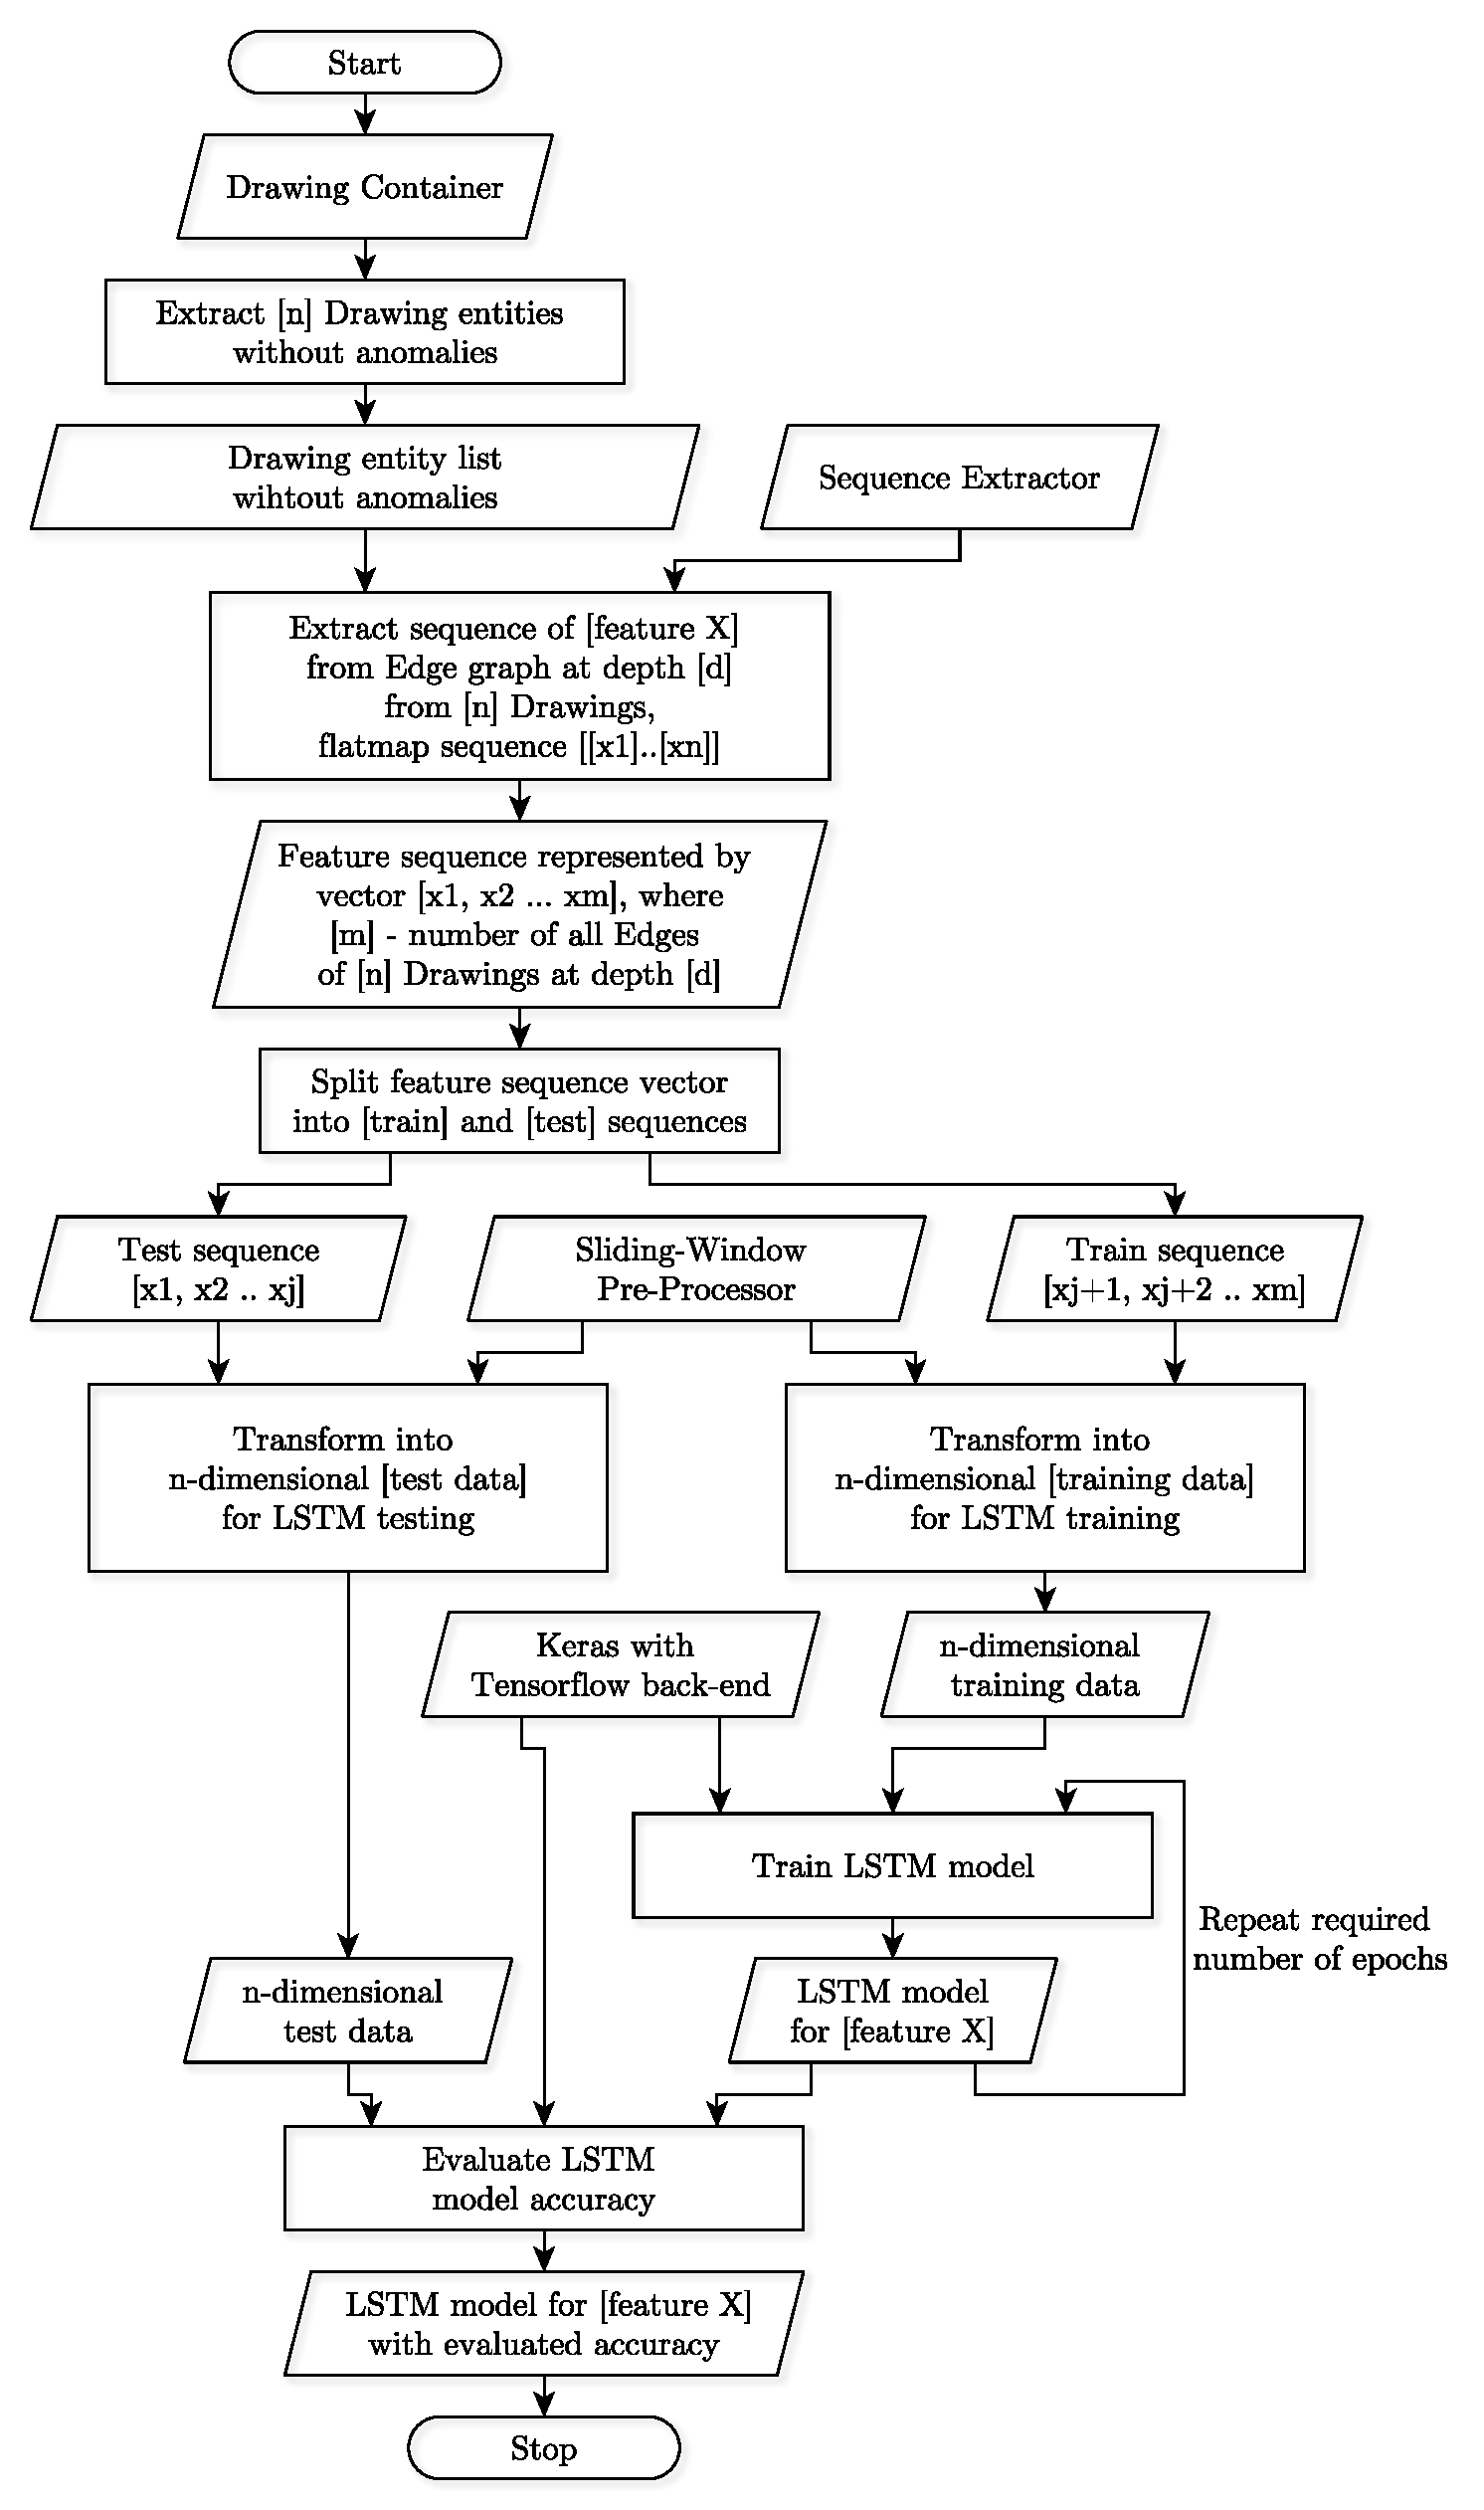
\includegraphics[width=0.90\textwidth]
        {images/anomaly/flow-lstm-training}
    \caption{\textit{LSTM Model} Training --- Flow Diagram}
    \label{flow-lstm-training}
\end{figure}

\section{Anomaly Detection}

By definition, anomaly detection process usually refers to the problem of finding sequences in data, that do not conform to expected behavior. 

Current algorithm utilizes most common Neural-Networks-Based \textit{anomaly detection} method, described by \citet*{chandola2009anomaly}. Main idea is to initially predict a sequence from its previous samples and then decide whether the element of sequence is \textit{anomaly} or \textit{normal}, based on prediction \textit{error}, or in other words --- an \textit{anomaly} is an element, which cannot be predicted from the past normal time-series or sequential data using trained \textit{NN} model. 

\textit{First part of the method} --- is already implemented: neural network, in current context --- \textit{LSTM} model is trained on the \textit{normal} sequential dataset to learn the \textit{normal} behaviour of the sequence, or to \textit{accurately} predict $x_{i+1}$ next value of the sequence from $[x_{i-n}, ...x_{i-1}, x_i]$ previous $n$ values, if \textit{normal}, i.e., \textit{non-anomaly} input were supplied.

\textit{Second part of the method} --- is described in current chapter: each test instance, in our case --- feature-sequence extracted from the \textit{Drawing} entity, is provided as an input to the LSTM neural network model. If model predicts each next element of the sequence with error below certain \textit{threshold}, this particular element is treated as \textit{normal}. If measured error is above pre-defined \textit{threshold} --- element doesn't conform to expected behaviour of the sequence, hence treated as \textit{anomaly}.

\begin{comment}

Anomaly detection refers to the problem of finding patterns in data that do not conform
to expected behavior. These nonconforming patterns are often referred to as anomalies

At an abstract level, an anomaly is defined as a pattern that does not conform to
expected normal behavior. A straightforward anomaly detection approach, therefore,
is to define a region representing normal behavior and declare any observation in the
data that does not belong to this normal region as an anomaly

Neural networks have been applied to anomaly detection in multi-class as well as oneclass
settings. A basic multiclass anomaly detection technique using neural networks operates in
two steps. First, a neural network is trained on the normal training data to learn the
different normal classes. Second, each test instance is provided as an input to the neural
network. If the network accepts the test input, it is normal and if the network rejects
a test input, it is an anomaly 


Current process utilizes recently created LSTM neural network for sequence modelling and expected value prediction, based on the immediate input of the 
Following steps are executed to detect unexpected elements within arbitrary feature sequence.  General idea of the process is to reproduce normal signal

% Instead, they first predict a sequence from its past samples and then determine whether the sequence is an anomaly or not based on the prediction error, i.e., an anomaly is an event, which cannot be predicted from the past nominal data.

Thus, they require a probabilistic model for the prediction
error and a threshold on the probabilistic model to detect
anomalies, which results in challenging optimization problems
and restricts their performance accordingly [1], [15], [16].
Furthermore, both the common and neural networks based
approaches can process only fixed length vector sequences,
which significantly limits their usage in real life applications
[1].

\end{comment}

\subsection{Anomaly Entity}

In current context, \textit{anomaly} --- is an element of a feature-sequence, i.e, certain feature instance of the certain \textit{Edge} of the Drawing object. Intuitively, \textit{anomaly} refers to both \textit{feature} and \textit{Edge} instances, thus it was decided to design \textit{Anomaly} entity in order to wrap \textit{meta-information} about feature name, predicted and actual values, also to establish a link to related \textit{Edge} object by storing its \textit{reference}. Current design approach takes advantage of already existing flexible data-structure of Drawing graph by decorating its \textit{Edge} elements with extracted \textit{Anomaly} objects.

\subsection{Anomaly Detection Process}

Certain subset of $n$ feature-types was already pre-defined, and $n$ neural network \textit{LSTM models} were trained to predict corresponding feature-sequences. Similarly, current anomaly detection process is executed for single Drawing object $n$ times for each pre-defined feature-sequence and optionally produces Anomaly objects, which are stored in graph data-structure of Drawing entity for successive Anomaly-type feature generation and analysis. Process is illustrated on flow diagram on Figure \ref{flow-anomaly-detection} and consists of following steps:

\begin{easylist}

& \textit{Sequence Extraction} --- with \textit{Sequence Extractor} component, obtain sequence for particular feature $x$ of Drawing instance. Sequence is represented by vector of $[x_1, x_2...x_n]$, where $n$ -- is number of $Edges$ at deepest available depth $d$ = 4 of Edge graph.

& \textit{LSTM Input Generation} --- with \textit{Sliding-Window Pre-Processor} component transform training $[x_1, x_2...x_n]$ sequence into n-dimensional data in the form of tuple vectors $[(a_1, b_1), ..., (a_i, b_i),...(a_m, b_m)]$, where $a_i$ itself is a vector with $n$ values $a_i = [x_{i-n}, ...x_{i-1}, x_i]$, and $b_i$ is singular value $b_i = x_{i+1}$.

& \textit{Sequence Prediction} --- from \textit{LSTM Container} extract required \textit{LSTM model}, trained for feature $x$ sequence prediction. Feed generated n-dimensional data from \textit{Sliding-Window Pre-Processor} to \textit{LSTM model}, obtain predicted sequence, represented by vector of $[y_1, y_2...y_n]$.

& \textit{Error evaluation} --- subtract predicted sequence, represented by vector $[y_1, y_2...y_n]$ from original vector $[x_1, x_2...x_n]$ and apply $square$ function.
Obtain vector of errors $[e_1, e_2...e_n]$, so each element is \textit{squared standard error} $(SE)^2$ for original element $x_i$ of the sequence. 
Generated $[e_1, e_2...e_n]$ may include outlier-peaks (shown on third chart of the Figure \ref{anomaly}). Peaks are removed by applying \textit{Scipy} library standard \textit{median} filter function. Finally, locate anomalies --- elements with error $e_i$ above pre-defined threshold $t$, by retrieving corresponding indices of the sequence. 

&& \textit{Threshold calculation logic} --- threshold was calculated separately for each \textit{LSTM model}, during training process: feed model with \textit{normal} test data  $[a_1, a_2, ...a_n]$, obtain predicted sequence $[\hat{a_1}, \hat{a_2}, ...\hat{a_n}]$, evaluate \textit{mean squared error} \textit{MSE} with (\ref{mse}). Required threshold is calculated by $t = C \times MSE$, where hyper-parameter $C$ is defined for each model experimentally.

\begin{equation}
\label{mse}
  MSE = \frac{1}{n}\sum_{i=1}^{n} (a_i - \hat{a_i})^2
\end{equation}

& \textit{Anomaly Generation} --- after previous step, indices of anomalies $[i_1, i_2, ...i_m]$ within sequence $[y_1, y_2...y_n]$ are defined and correspond to \textit{Edge} object local indices at specified depth $d = 4$ of the \textit{Drawing} graph. Look-up and obtain \textit{Edge} entities by corresponding $i$ index. Wrap meta-information about feature \textit{type}, actual value $x_i$ and predicted value $y_i$ along with \textit{reference} to corresponding \textit{Edge} object by constructing \textit{Anomaly} entities. 

\end{easylist}

\begin{figure}[htb]
  \centering
    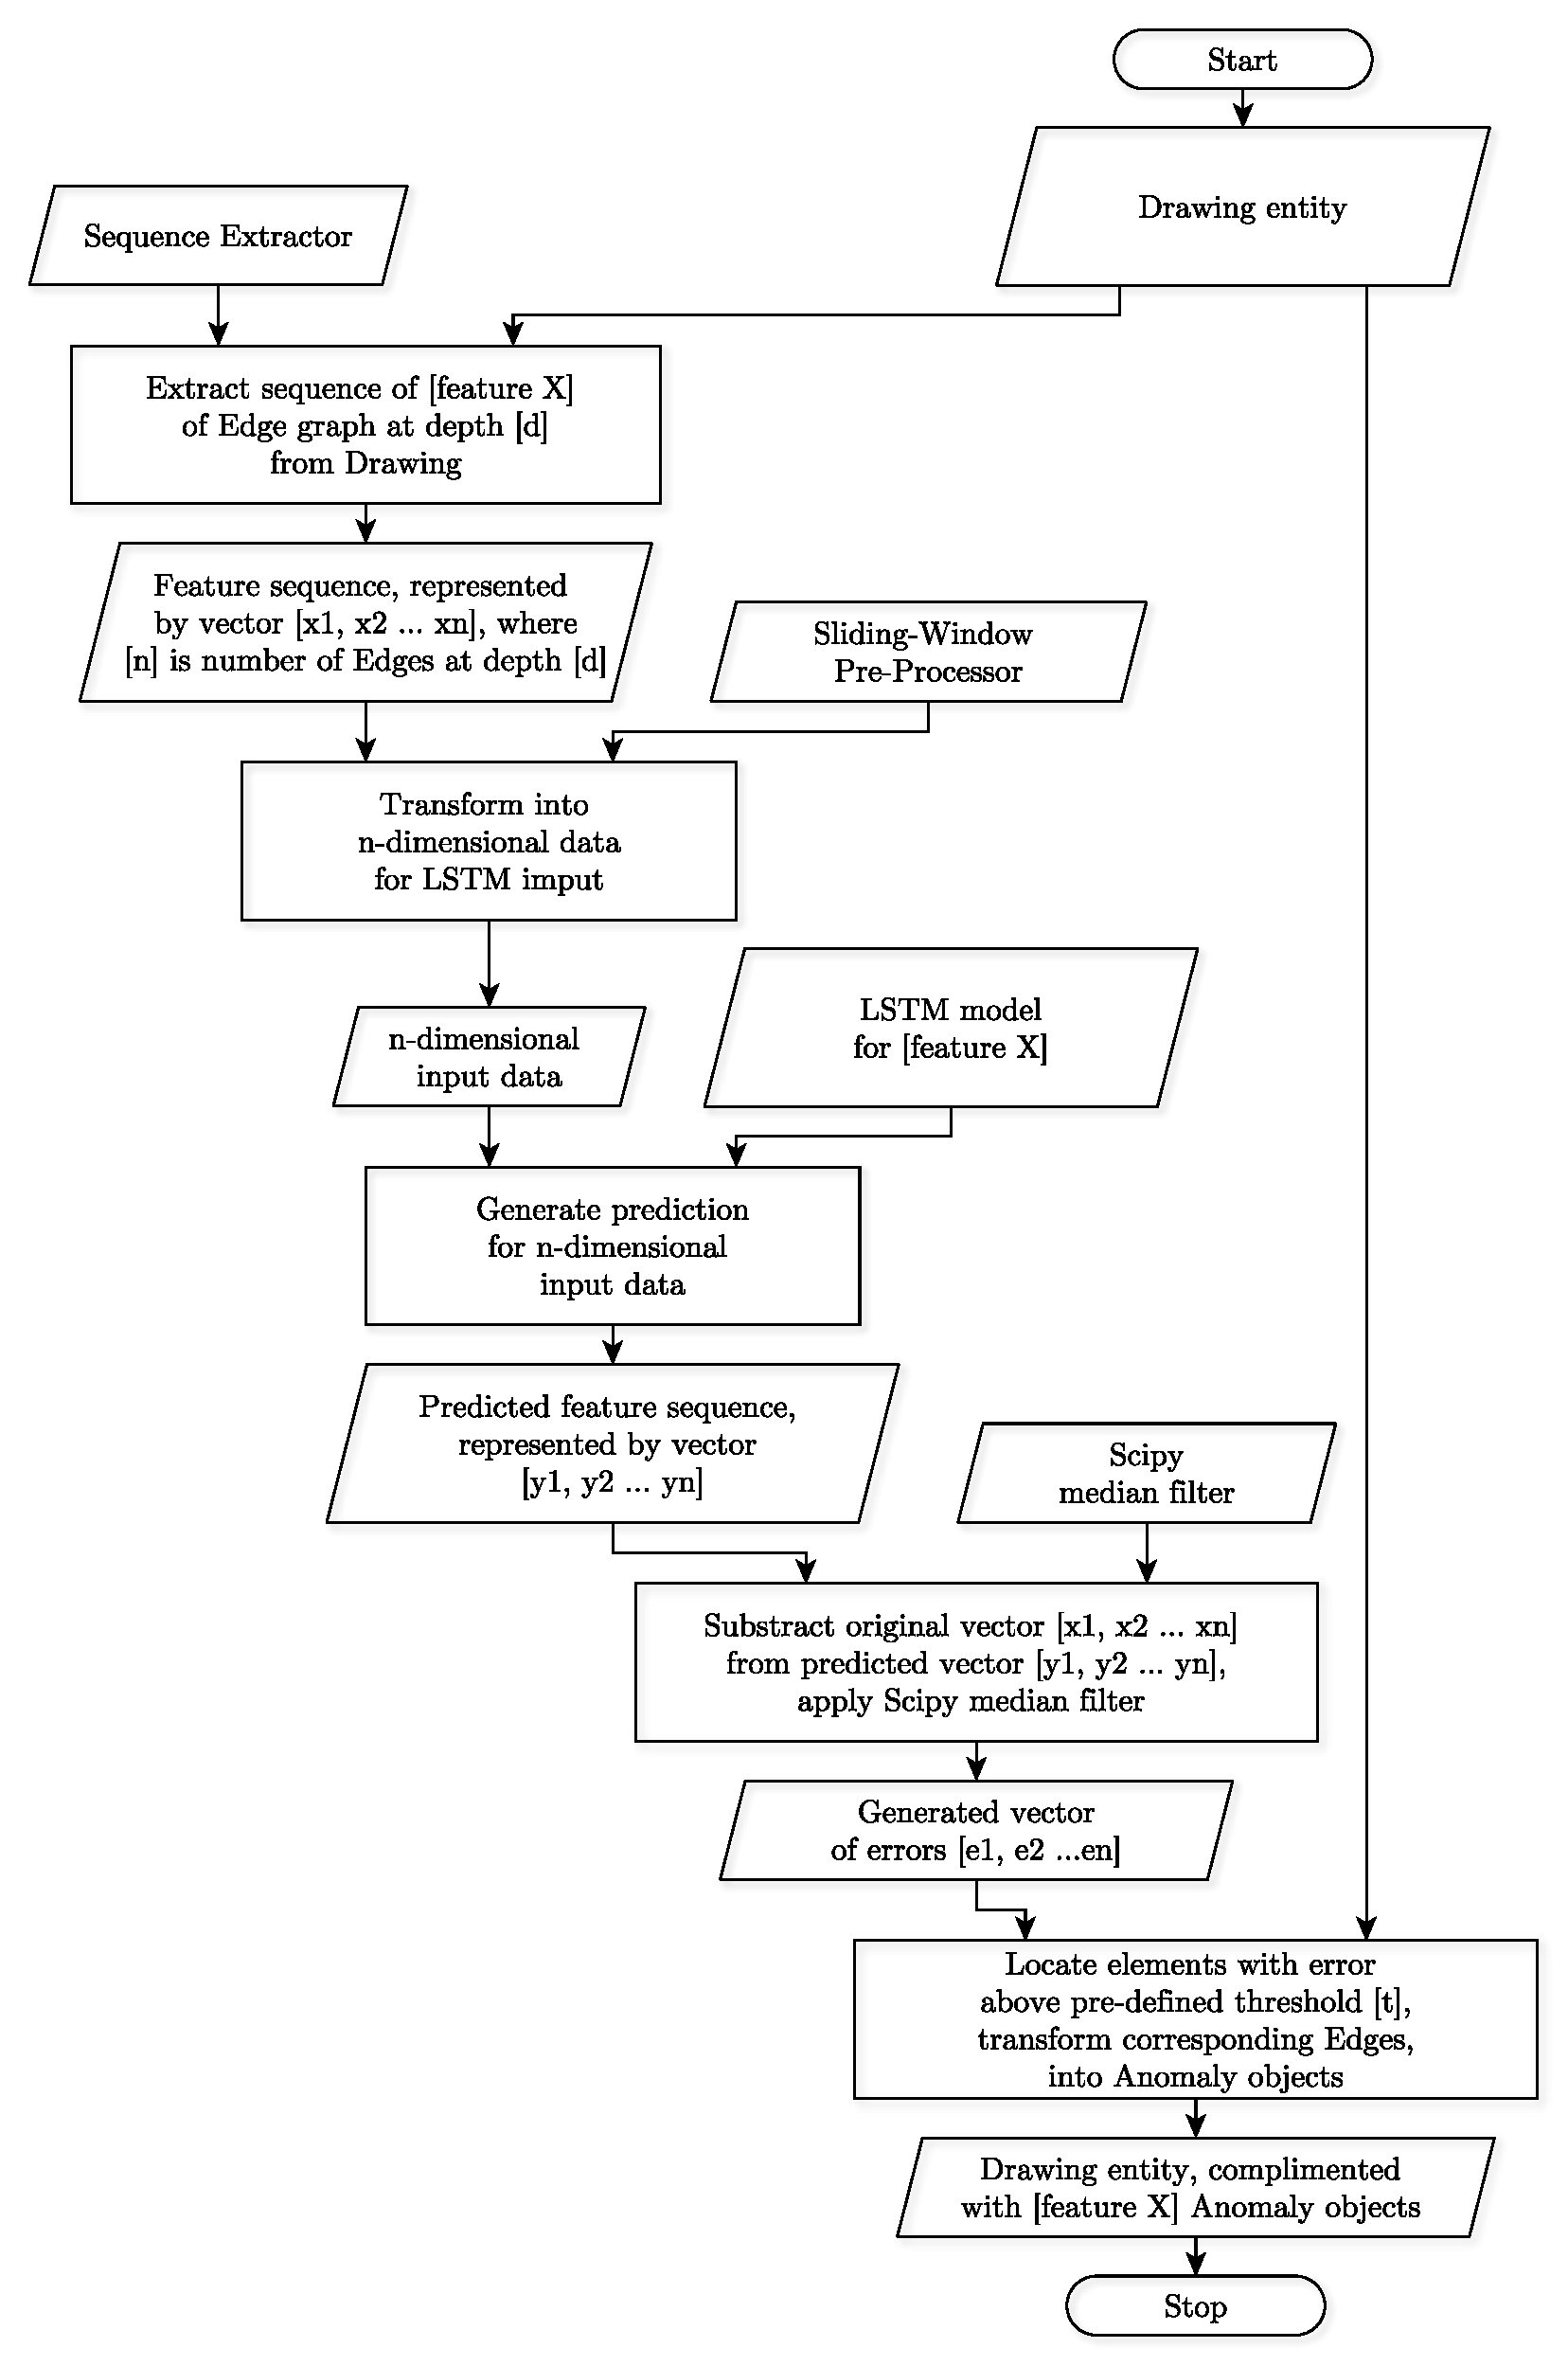
\includegraphics[width=0.99\textwidth]
        {images/anomaly/flow-anomaly-detection}
    \caption{Anomaly Detection Process --- Flow Diagram}
    \label{flow-anomaly-detection}
\end{figure}

\subsection{Anomaly Features}

It was pre-defined subset of $n$ feature-types $[t_1, t_2, ...t_n]$, extracted $n$ feature-sequences and trained $n$ \textit{LSTM models} to evaluate $n$ anomaly-types. Current work analyzes $n = 6$ feature-sequences \textit{[angle, pressure, length, duration, longitude, latitude]} of the Edge, i.e., sequences of mean values of \textit{[angle, pressure, length, duration, longitude, latitude]} within \textit{Edge} objects of \textit{Drawing} graph at depth $d = 4$.

It is feasible to recursively traverse whole graph and evaluate number of anomalies for each node of the graph at arbitrary depth level $d$. Feature extraction algorithm follows simple logic: 

\begin{easylist} [itemize]

& Obtain all \textit{Edges} objects $[e_1, e_2, ...e_m]$ of the \textit{Drawing} graph at depth $d$
& Recursively \textit{count} all anomalies for each of $[e_1, e_2, ...e_m]$ and feature-type $[t_1, t_2, ...t_n]$. 

& Evaluate output for depth $d = 0$, $d = 1$

& Construct feature names by combining prefix and suffix. \textit{Prefix} -- is taken from corresponding entity name with possible values of \textit{[Drawing, Edge\_1, Edge\_2, ...Edge\_n]}. \textit{Suffix} -- is matching name of the feature type for current anomaly -- \textit{[angle, pressure, length, duration, longitude, latitude]}.

% && For d = 0 name is Drawing, for d = 1 [Edge_1, Edge_2, ... Edge_n]

\end{easylist}

% We extract number of anomalies of each n = 6 types for each element at depth d = 0 and d =
% We produce anomaly feature by combining anomaly type and number of anomalies
% After last phase of the algorithm subset of Anomaly objects was obtained. Anomaly is wrapper-object with meta-information and reference to the Edge with same index and known depth d within Drawing graph. In theory it is possible to extract n features from n anomalies, by constructing relevant names from Edge index, depth and type. However to limit the scope of feature space it was decided produce features by counting anomalies within whole drawing and within edges at depth = 1
% Obtained \textit{Anomalies} are wrapper-objects around \textit{Edge} entities. Transitively they receive same characteristics of the Edge entity such as: interpret-ability and human-understandable. Flatten Anomaly object into scalar values - generate features Anomaly is wrapper object around Edge entity therefore is 


\section{Anomaly Detection Example}

Following Figure \ref{anomaly} shows example output of proposed \textit{anomaly detection} algorithm. Fourth chart represents Luria 'P' pattern in \textit{Cartesian} coordinates, drawn with \textit{mistakes}. Luria 'P' pattern by definition, should only contain vertical and horizontal lines. So only segments with angles with slight variation around values in subset of [90, 0, -90] are allowed. Pattern segments drawn at unexpected \textit{angle} (edges 2 and 13) with unexpected \textit{order} (edge 20) considered as \textit{anomalies}.

First chart on Figure \ref{anomaly} illustrates extracted sequence of Edge angles $[a_1,.. a_n]$ of \textit{Drawing} graph at depth $d = 4$. Second chart shows angle sequence $[\hat{a_1}, ...\hat{a_n}]$ predicted by corresponding \textit{LSTM model} trained to reproduce normal behaviour of Luria 'P' pattern. Third chart demonstrates error vector, or squared difference between $[a_1,.. a_n]$ and $[\hat{a_1}, ...\hat{a_n}]$, represented by $[e_1, ...e_n]$ with applied \textit{median} filter. Elements of the sequence $[e_1, ...e_n]$ above pre-defined threshold $t = C \times MSE$ marked as \textit{anomalies} and shown on all charts as \textit{gray circles}. Hyper-parameter for corresponding \textit{angle-related} \textit{LSTM model} is $C = 15$

\begin{figure}[htb]
  \centering
    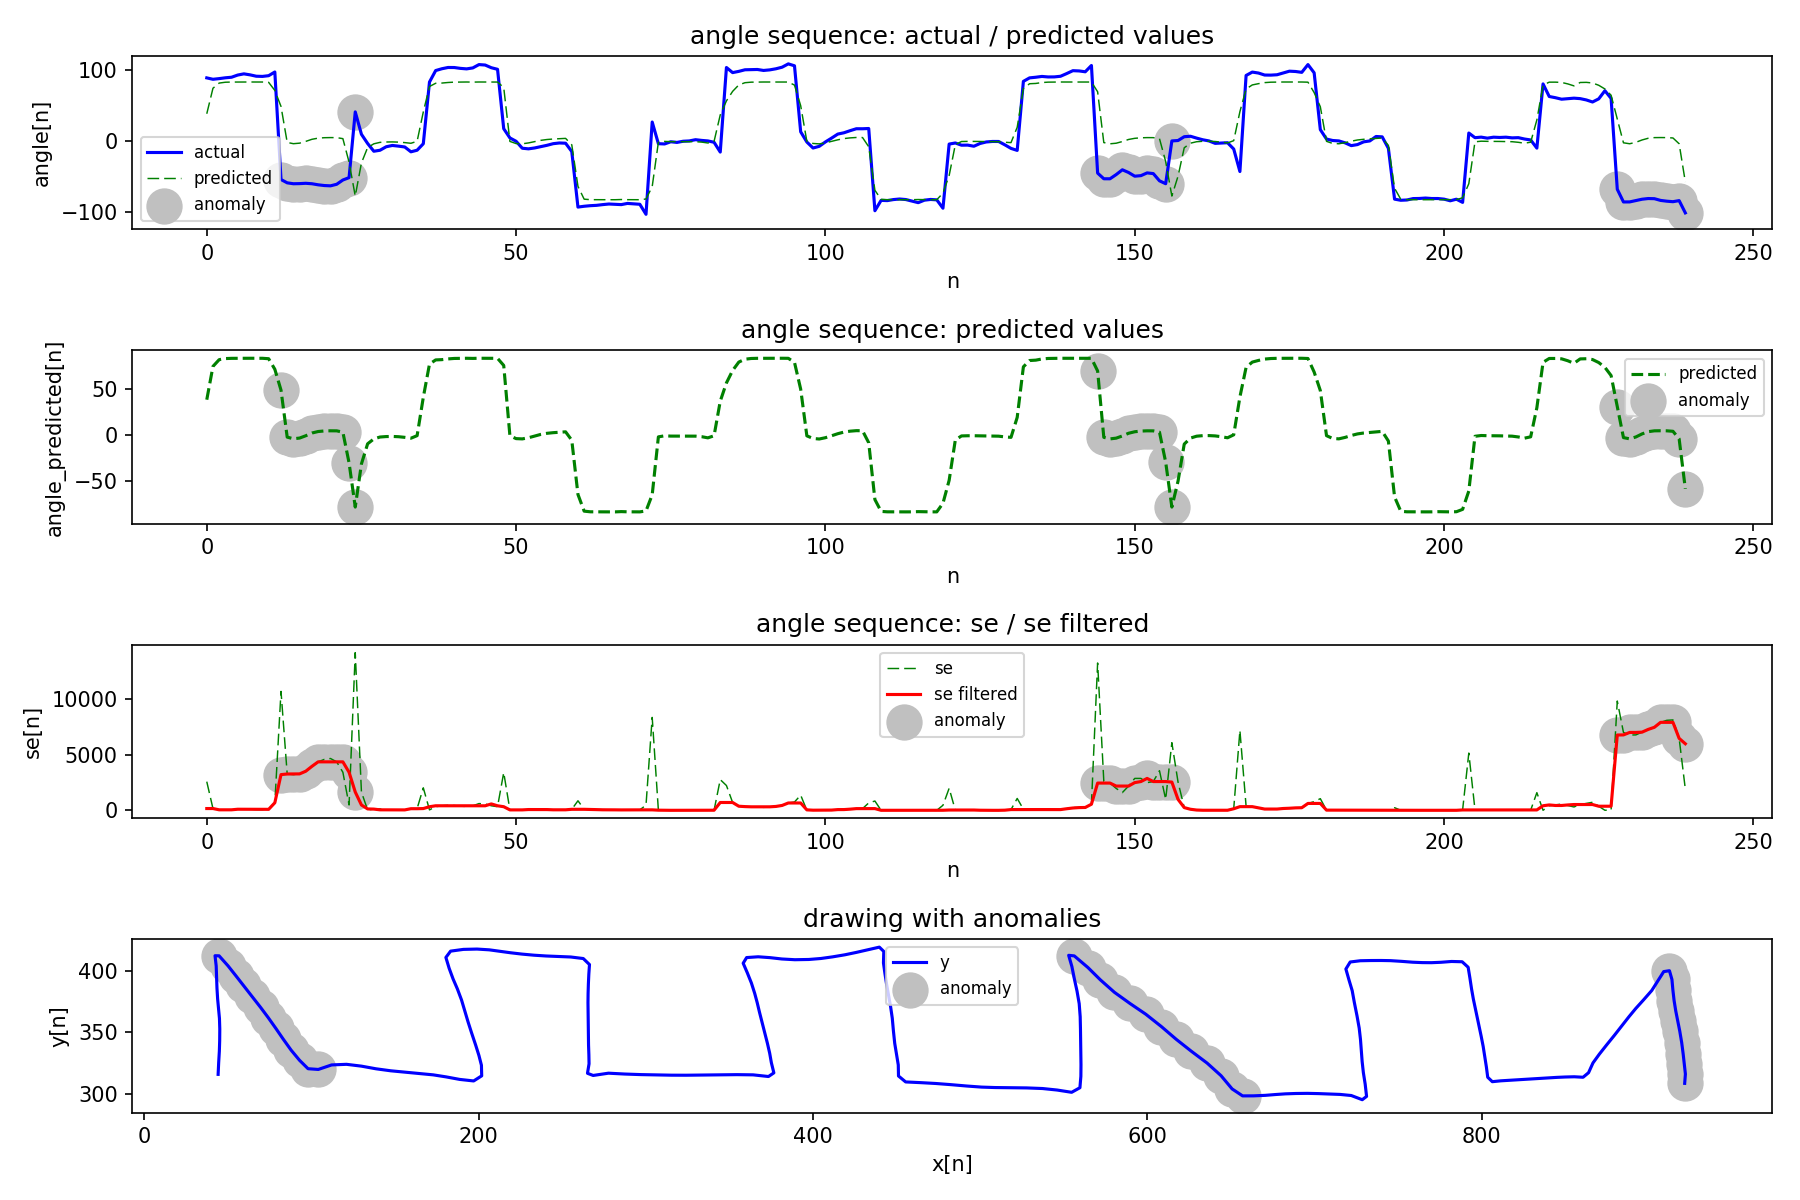
\includegraphics[width=0.99\textwidth]
        {images/anomaly/anomaly}
    \caption{Anomaly Detection --- Example Output}
    \label{anomaly}
\end{figure}


% Sample result of the algorithm is presented on Figure \ref{anomaly}
